\documentclass[a4paper, 12pt]{article}

%Paragraph jumps and indentation
\setlength{\parskip}{1.5em}
\setlength{\parindent}{1.25cm}

%Border
\usepackage[left=1in, right=1in, top=1in, bottom=1in]{geometry}

%Double spacing
\usepackage{setspace}
\doublespacing

%Packages
\usepackage{amsmath}
\usepackage[dvipsnames]{xcolor}
\usepackage{mathtools}
\usepackage{amsfonts}
\usepackage{titlesec}

%Images
\usepackage{graphicx}
\graphicspath{ {./images/} }
\usepackage{wrapfig}
\usepackage{float}

%Tables
\usepackage{multirow}
\usepackage{array}
\usepackage{tabu}
\titleformat{\section}
{\normalfont\large\bfseries}{\thesection}{1em}{}
\titleformat{\subsection}
{\normalfont\large\bfseries}{\thesubsection}{1em}{}

%Equation numbering
\counterwithin{equation}{section}

%Links
\usepackage{hyperref}
\urlstyle{same}

%Diagrams
\usepackage{pgfplots}
\pgfplotsset{compat=newest}
\usetikzlibrary{positioning, arrows.meta}
\usepgfplotslibrary{fillbetween}
\usepackage{wrapfig}


\begin{document}

\begin{titlepage}
  \begin{center}
    \textbf{IB ECONOMICS} \hspace{1cm} STANDARD LEVEL\\
    \vspace*{3cm}
    \textbf{Title of the article:}
    Mozambique approves investment projects
    valued at about US\$5 billion in H1 2025\\

    \textbf{Source of the article:}
    African Mining Market\\

    \textbf{Link to the article:}
    \url{https://africanminingmarket.com/mozambique-approves-investment-projects-valued-at-about-usd5-billion-in-h1-2025}\\

    \textbf{Article publish date:}
    September 1, 2025\\

    \textbf{Article access date:} September 11, 2025\\

    \textbf{Commentary writing date:} September 11, 2025\\

    \textbf{Unit of the syllabus:}
    Macroeconomics\\

    \textbf{Key concept:}
    Intervention.\\

    \vfill
    Word count: 186
  \end{center}
\end{titlepage}

\section*{Extract}
{ \itshape
  {\large The Mozambican government has approved 115 investment projects valued at about US\$5 billion in the first half of 2025, with the potential to create 17,000 jobs. Prime Minister Benvinda Levi announced the figures on 30th August, at the closing of the 60th Maputo International Fair (FACIM).}

  The largest project is Green Energy Mozambique, a US\$3 billion industrial park in Sofala province. The complex is expected to generate 10,000 direct jobs and boost production of key materials including aluminum, steel, cement, batteries, and solar panels.

  More than 88\% of total investment was directed to Sofala, far ahead of Maputo. Foreign capital accounted for US\$3.2 billion, with contributions from investors in 25 countries. The funds mainly target industry, transport, communications, and services. Domestic investment stood at US\$144 million.

  Levi said the results show the Mozambican economy is rebounding after climate shocks and post-election tensions, with the private sector driving growth. She also highlighted the launch of a US\$250 million mutual guarantee fund during the fair to support recovery and expand private sector participation.

  These achievements align with the country's strategy to strengthen investor appeal. In recent years, Mozambique has pursued reforms to attract capital, including the creation of the Investment and Export Promotion Agency (APIEX) and the adoption of a new investment law in 2023. The country now offers tax and customs incentives, along with special economic zones in agriculture, aquaculture, and less-developed regions.

  According to UNCTAD, Mozambique ranked fourth in Africa for foreign direct investment inflows in 2024, reaching US\$3.55 billion, up from US\$2.5 billion in 2023, when it placed sixth.

}

\newpage
\section*{Commentary}

In summary, Mozambique has approved major new investment projects worth about US\$5 billion, mostly foreign-funded and centered in Sofala, including a large green energy park producing commodities and solar panels.
The initiatives are expected to create jobs and support the country's economic recovery after recent shocks, with reforms and incentives aimed at strengthening investor confidence.
This commentary will discuss how \textbf{intervention} by the government through this form of fiscal policy achieves its effects on increasing economic growth and decreasing unemployment.
The analysis shall be done with respect to the Keynesian model of aggregate demand and supply.

\begin{wrapfigure}{L}{0.6\textwidth}
  \begin{center}
    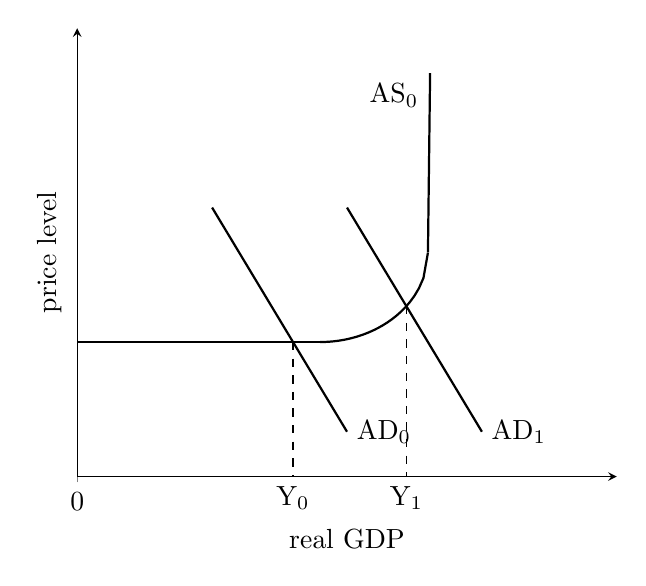
\begin{tikzpicture}[scale=1]
      \begin{axis}[
          axis lines=left,
          xlabel={real GDP},
          ylabel={price level},
          xmin=0, xmax=1,
          ymin=0, ymax=1,
          xtick={0}, ytick={\empty},
          clip=false
        ]

        \addplot[thick, domain=0:0.45] {0.3};
        \addplot[thick, domain=0.45:0.65] {0.5 - sqrt(1/25 - (x-0.45)^2)};
        \addplot[thick, domain=0.65:0.654] {100*x - 64.5};
        \node[left] at (0.65, 0.85) {AS$_0$};

        \addplot[thick, domain=0.25:0.5] {1.1-2*x};
        \node[right] at (0.5, 0.1) {AD$_0$};

        \addplot[thick, domain=0.5:0.75] {1.6-2*x};
        \node[right] at (0.75, 0.1) {AD$_1$};

        \draw[dashed] (0.4, 0.3) -- (0.4, 0);
        \node[below] at (0.4, 0) {Y$_0$};

        \draw[dashed] (0.61, 0.38) -- (0.61, 0);
        \node[below] at (0.61, 0) {Y$_1$};

      \end{axis}
    \end{tikzpicture}
    \caption{Increase in AD}
  \end{center}
\end{wrapfigure}





\begin{figure}[h]
  \begin{center}
    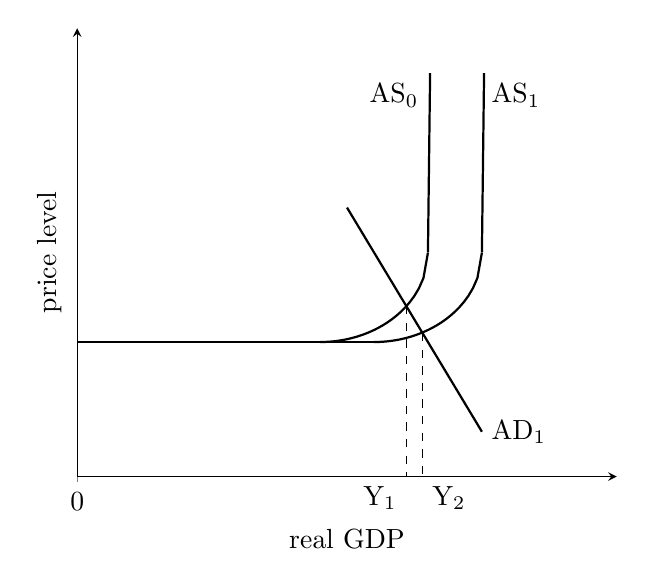
\begin{tikzpicture}[scale=1]
      \begin{axis}[
          axis lines=left,
          xlabel={real GDP},
          ylabel={price level},
          xmin=0, xmax=1,
          ymin=0, ymax=1,
          xtick={0}, ytick={\empty},
          clip=false
        ]

        \addplot[thick, domain=0:0.55] {0.3};
        \addplot[thick, domain=0.55:0.75] {0.5 - sqrt(1/25 - (x-0.55)^2)};
        \addplot[thick, domain=0.75:0.754] {100*x - 74.5};
        \node[right] at (0.75, 0.85) {AS$_1$};

        \addplot[thick, domain=0.45:0.65] {0.5 - sqrt(1/25 - (x-0.45)^2)};
        \addplot[thick, domain=0.65:0.654] {100*x - 64.5};
        \node[left] at (0.65, 0.85) {AS$_0$};

        \addplot[thick, domain=0.5:0.75] {1.6-2*x};
        \node[right] at (0.75, 0.1) {AD$_1$};


        \draw[dashed] (0.61, 0.38) -- (0.61, 0);
        \node[below left] at (0.61, 0) {Y$_1$};

        \draw[dashed] (0.64, 0.32) -- (0.64, 0);
        \node[below right] at (0.64, 0) {Y$_2$};

      \end{axis}
    \end{tikzpicture}
    \caption{Increase in AS}
  \end{center}
\end{figure}


Direct impact on demand: G and I component of AD. (don't mention exports here)

(Perhaps mainly in terms of quantification) interventionist SS policy, as industrial policy creating jobs and also in favor of `green energy'.

``The country now offers tax and customs incentives, along with
special economic zones in agriculture, aquaculture, and less-developed regions, 
[...]

support recovery and expand private sector participation.'' (Market based SS policy)

Mozambique GDP: 22.42B USD

\end{document}